% !TeX root = document.tex
% !TeX encoding = UTF-8 Unicode

\chapter{Resultados e Discussões}%
\label{chp:results}

Neste capítulo são apresentados os resultados parciais obtidos, separados por
tópicos conforme o cronograma apresentado na proposta.

\section{Estudos teóricos}%
\label{sec:studies}

\subsection{Controle preditivo por modelo}%
\label{subsec:mpc-studies}

O livro-texto utilizado para os estudos do controle preditivo por modelo foi o
do~\textcite{book:wang}, com as outras referências sendo usadas de forma
complementar. Para a execução deste projeto propõe-se o estudo dos capítulos 1 a
4, que tratam do caso discreto.

Foram estudados os capítulos 1 e 2, que apresentam o conceito do controlador e a
formulação com restrições, respectivamente. Como os estudos teóricos de \ac{MPC}
foram iniciados antes da alteração da eletrônica do forno, a técnica foi testada
utilizando os tanques comunicantes (Figura~\ref{fig:tanks}) presentes no
Laboratório de Sinais e Sistemas.

\begin{figure}[ht!]
    \centering
    \captionsetup{justification=centering}
    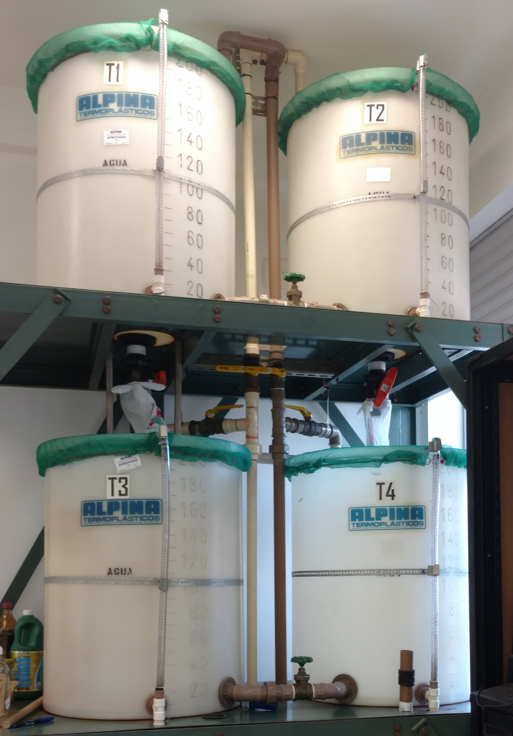
\includegraphics[height=0.5\linewidth]{imgs/tanques}
    \caption{Sistema de tanques comunicantes}%
    \label{fig:tanks}
\end{figure}

Os tanques utilizados são o 1º e 2º, que estão localizados na parte superior e
marcados como T1 e T2. A bomba insere água no primeiro tanque e esta escoa para
o segundo através de uma válvula localizada na parte inferior. A água é então
removida através de uma válvula no fundo do tanque 2. O objetivo de controle é
o nível do tanque 2.

Uma simulação do controlador MPC controlando o modelo desse sistema pode ser
visto na Figura~\ref{fig:mpc-simulated}. Observa-se que o sinal de controle é
mantido em 100\% por quase todo o transitório, e é então abaixado para o valor
de equilíbrio, fazendo com que o tanque encha de forma rápida mas minimizando o
overshoot.

\begin{figure}[ht!]
    \centering
    \captionsetup{justification=centering}
    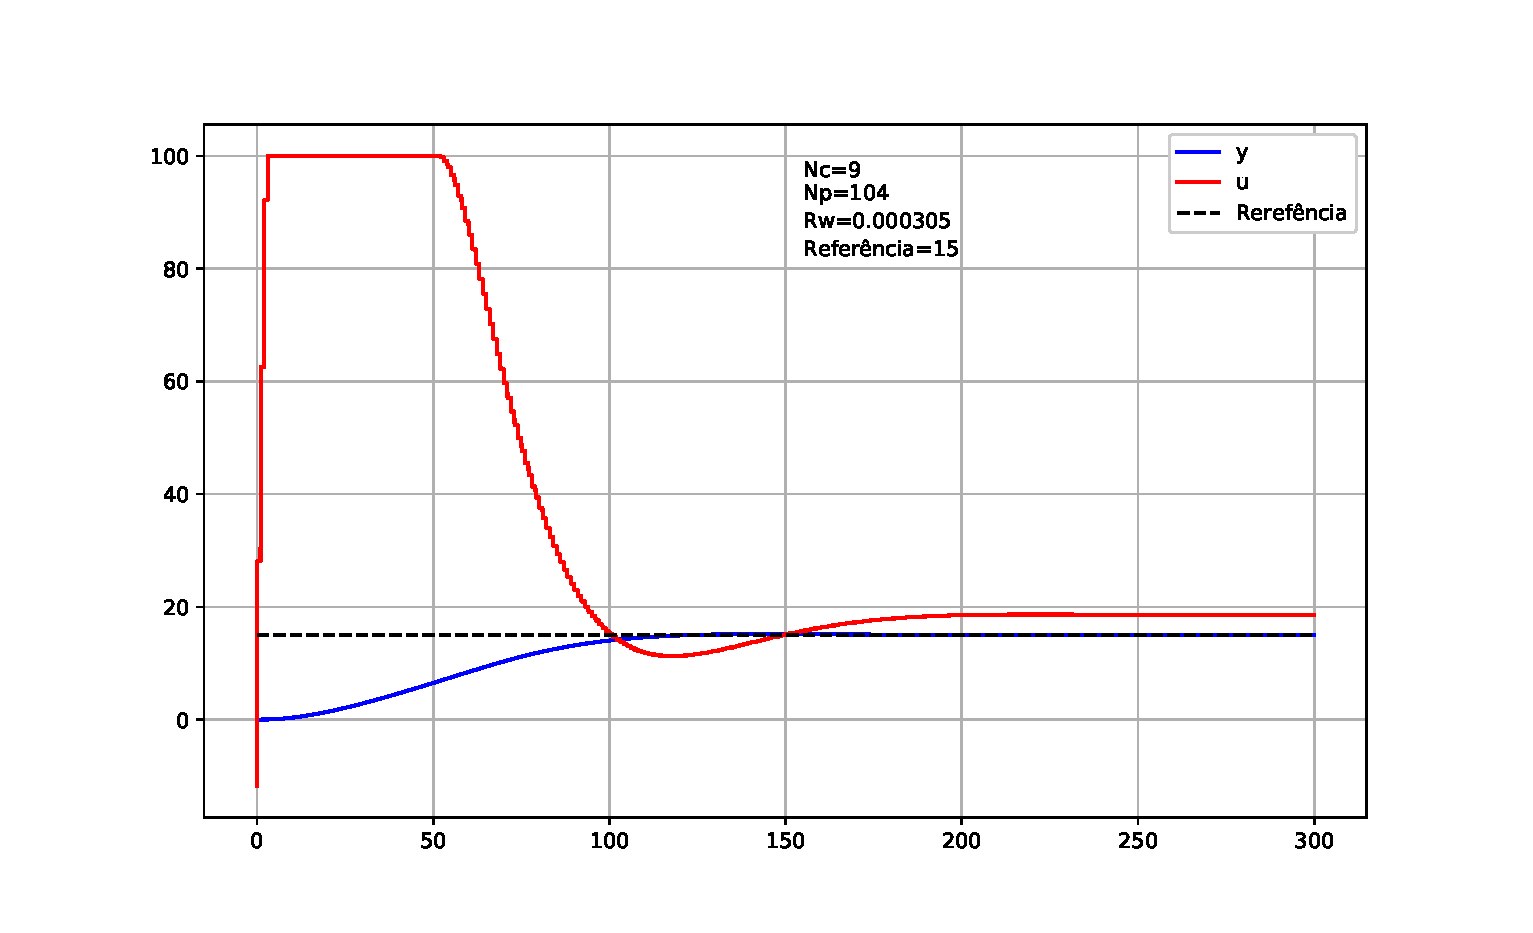
\includegraphics[height=0.5\linewidth]{imgs/mpc-simulado}
    \caption{Simulação do modelo dos tanques com controlador MPC}%
    \label{fig:mpc-simulated}
\end{figure}

Ao inserir este controlador no sistema real (Figura~\ref{fig:mpc-tanks})
obtem-se uma resposta parecida com a da simulação, porém mais lenta. Essa
diferença pode ser explicada por erro de modelagem e pelo fato que o sistema
real não é linear, sendo o modelo linearizado. No entanto a resposta continua
satisfatória.

\begin{figure}[ht!]
    \centering
    \captionsetup{justification=centering}
    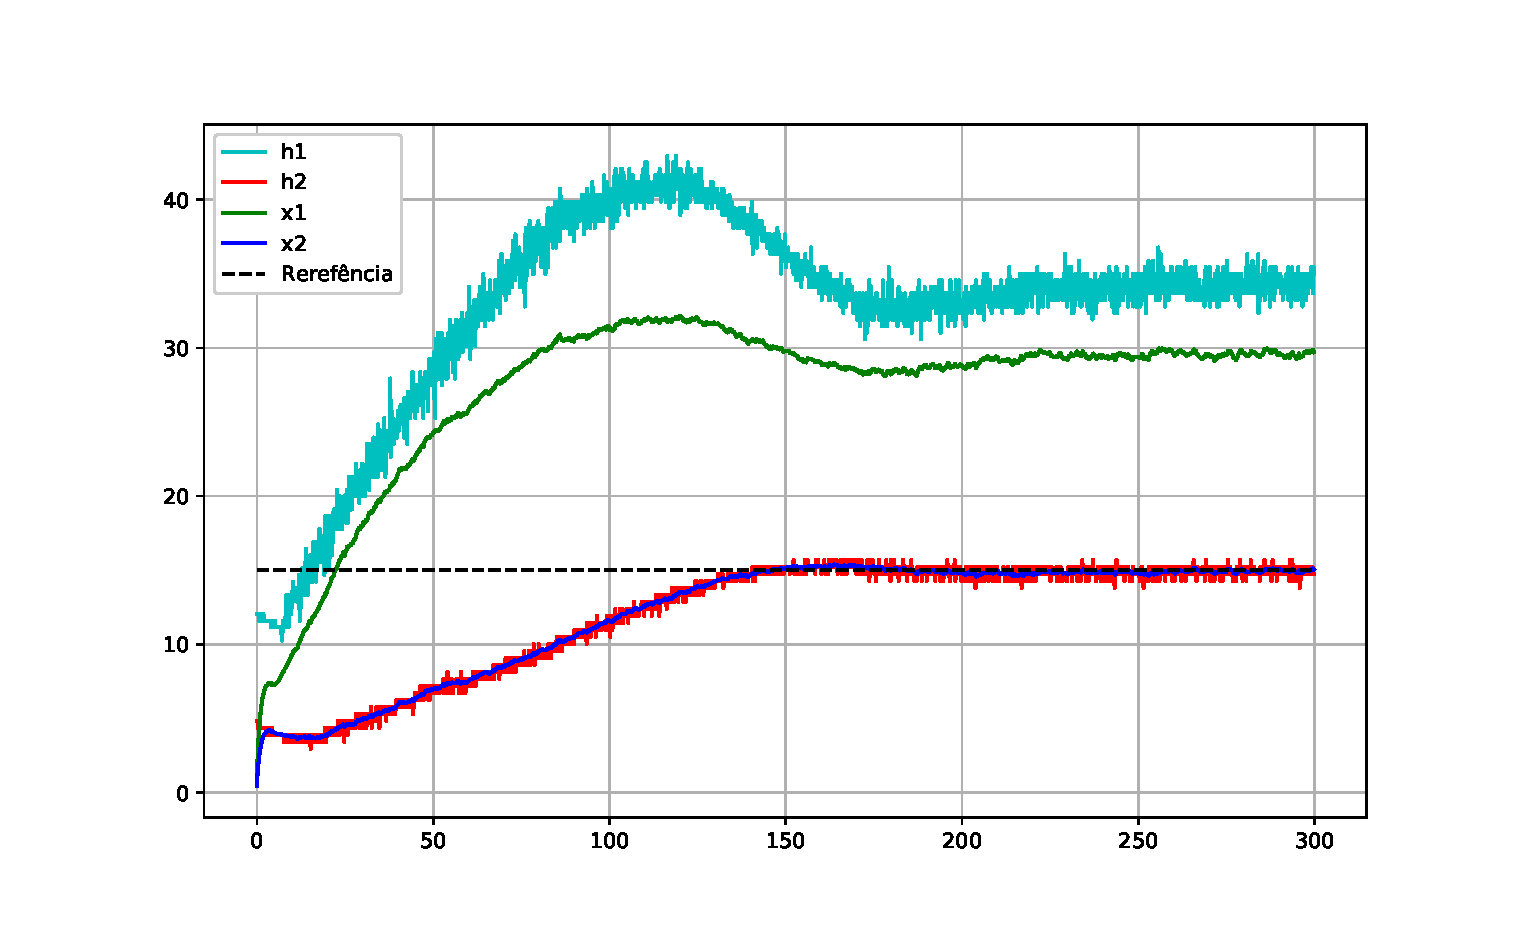
\includegraphics[height=0.5\linewidth]{imgs/mpc-tanque}
    \caption{MPC aplicado ao sistema real}%
    \label{fig:mpc-tanks}
\end{figure}

Como foi utilizado um observador, também pode-se perceber os efeitos do erro de
modelagem. Os estado estimado, \( x_1 \), embora apresente a mesma dinâmica, não
apresenta o mesmo ganho que o estado real, \( h_1 \). É interessante notar, no
entanto, que esta diferença não atrapalha o controlador, que continua capaz de
seguir a referência.

\subsection{Modelagem térmica e SPD}%
\label{subsec:spd-studies}

Os resultados obtidos por~\textcite{masterthesis:nelson} foram simulados e
utilizou-se o modelo \ac{SPD} apresentado com os observadores de Kalman e
exponencial com fator de esquecimento. Foi possível ver nos estados a saída
variando conforme a distância do atuador aumenta, como pode ser visto na
Figura~\ref{fig:spd-sim}. Os observadores também estimam com precisão os estados
do sistema simulado, conforme Figura~\ref{fig:spd-obs}.

\begin{figure}[ht!]
    \centering
    \captionsetup{justification=centering}
    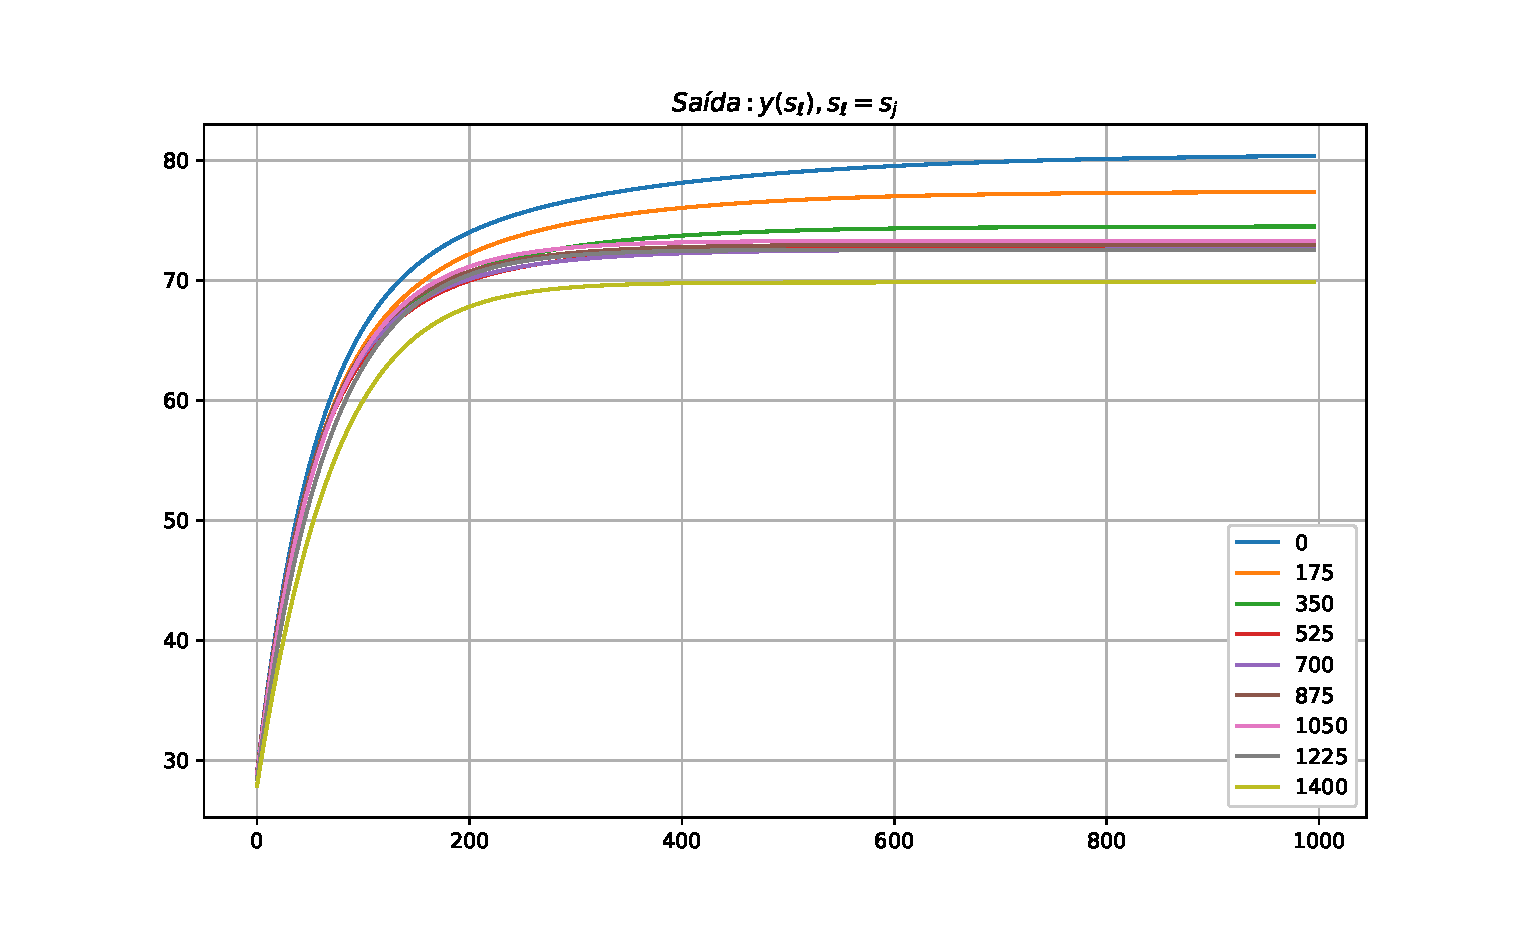
\includegraphics[height=0.5\linewidth]{imgs/spd-sim}
    \caption{SPD simulado}%
    \label{fig:spd-sim}
\end{figure}

\begin{figure}[ht!]
    \centering
    \captionsetup{justification=centering}
    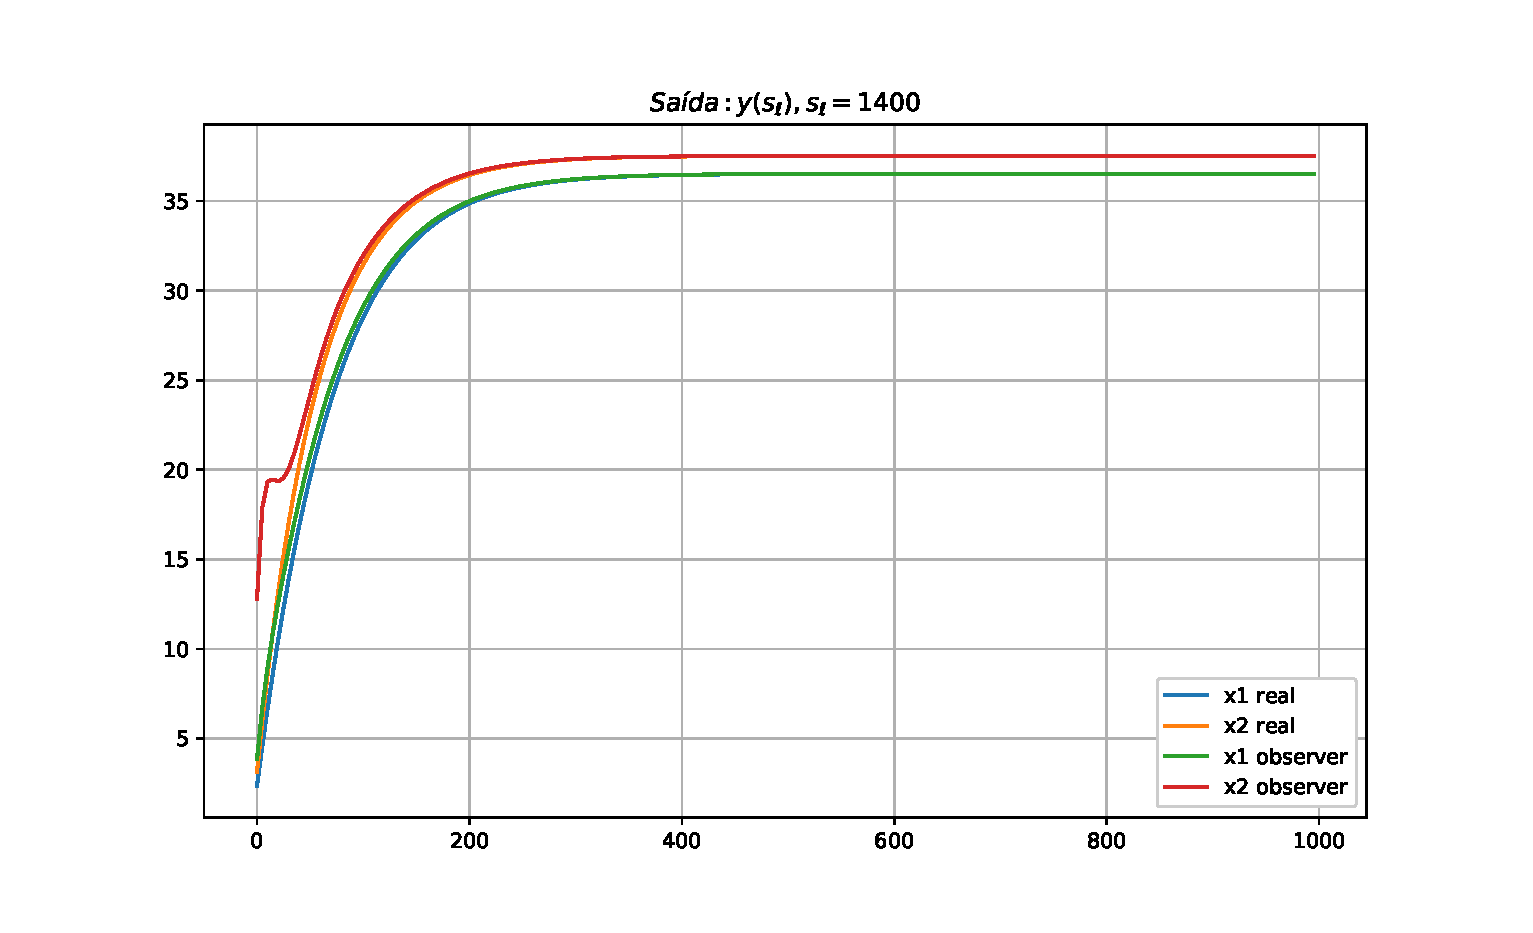
\includegraphics[height=0.5\linewidth]{imgs/spd-obs}
    \caption{SPD simulado com observador exponencial}%
    \label{fig:spd-obs}
\end{figure}

\section{Modificação do hardware e implantação da plataforma}%
\label{sec:hardware-and-plataform}

Ao estudar o circuito de acionamento e sensoriamento percebeu-se que não há a
necessidade de alterar o circuito. Devido a forma como o mesmo está montado, foi
necessário apenas a reprogramação dos microcontroladores presentes para
possibilitar a comunicação direta através de cabos USB.\ Após a reprogramação
foi possível acionar o circuito de potência e ler os valores dos sensores.

A instalação do Raspberry não foi feita pois o mesmo não foi adquirido a tempo.
No entanto, as modificações necessárias para a sua inserção já foram executadas
em outros projetos. Tais modificações compreendem principalmente mudanças no
software \textit{moirai} e já foram publicadas.

\section{Calibrações, testes e certificações}%
\label{sec:calibration}

O funcionamento do circuito eletrônico foi feito primeiramente acionando o
sistema desenvolvido por~\textcite{masterthesis:nelson}. Após verificar que este
era capaz de acionar as resistências e ler valores de todos os sensores foi
feita a modificação dos códigos dos microcontroladores e testou-se novamente com
o novo código. Verificou-se a necessidade de recalibrar os sensores e
reordená-los, identificando qual estava conectado a qual porta. Devido a forma
como se dá o acionamento não é necessária a calibração dos atuadores.

Para a calibração dos sensores foi utilizada uma garrafa térmica perfurada e um
ferro de solda. O mesmo foi ligado e foram feitas medições das temperaturas dos
sensores bem como de um termômetro industrial a cada 10 segundos. Foram
coletados 160 pontos. Utilizou-se então a técnica do mínimos quadrados para
encontrar uma expressão de correção linear, \( ax+b \), cujos coeficientes podem
ser vistos na Tabela~\ref{tbl:calib-coefs}.

\begin{table}[ht!]
    \centering
    \caption{Coeficientes da calibração}%
    \label{tbl:calib-coefs}
    \begin{tabular}{ccccccccccc}
          & S1    & S2   & S3   & S4   & S5   & S6   & S7   & S8   & S9   & S10  \\
        a & 0.85  & 0.82 & 0.82 & 0.78 & 0.79 & 0.83 & 0.76 & 0.74 & 0.81 & 0.79 \\
        b & -0.65 & 3.32 & 3.40 & 3.06 & 4.96 & 2.12 & 5.24 & 6.21 & 1.39 & 4.55
    \end{tabular}
\end{table}

A validação dos modelos e observadores ainda está sendo executada, pois foram
encontradas dificuldades durante a validação. O problema encontrado é que o
observador não está estimando o segundo estado corretamente. O proponente
buscará resolver este problema juntamente com seu orientador e o author do
modelo.

\section{Melhorias na plataforma}%
\label{sec:platform-enhancements}

Foram feitas várias modificações na plataforma. A lista completa pode ser vista
nos \textit{commits} de cada projeto, publicados desde 1º de março de 2018:

\begin{itemize}
    \item Lachesis: \url{https://github.com/acristoffers/Lachesis/commits/master}
    \item moirai: \url{https://github.com/acristoffers/moirai/commits/master}
    \item ahio: \url{https://github.com/acristoffers/ahio/commits/master}
\end{itemize}

As modificações que se destacam são:

\begin{itemize}
    \item implementação de um mecanismo de \textit{backup} de todo o banco,
    \item implementação de imporatação e exportação de configuração de hardware,
    \item seleção das variáveis a serem exibidas em gráficos,
    \item opção de clonar um teste ou controlador,
    \item melhoria da forma de apresentação de erros no terminal,
    \item melhoria de velocidade na recuperação de dados do banco,
    \item inserção de um novo banco de dados: MySQL (necessário no Raspberry),
    \item implementação de busca por drivers (ahio) em caminhos arbitrários.
\end{itemize}
